\documentclass[a4paper,10pt]{article}

\usepackage[english]{babel}
\usepackage{graphicx}
\usepackage[colorlinks, linkcolor=black, citecolor=black, urlcolor=black]{hyperref}
\usepackage{geometry}
\geometry{tmargin=2cm, bmargin=2cm, lmargin=2cm, rmargin=2cm}
\usepackage{todonotes} %Used for the figure placeholders
\usepackage{ifthen}

% Your name and student number must be filled in on the title page found in
% titlepage.tex.

\begin{document}
\newboolean{anonymize}
% Uncomment to create an anonymized version of your report
%\setboolean{anonymize}{true}

\input{titlepage}

\tableofcontents
\newpage

\section{Feature Representation}

The goal of this assignment is to classify face images into three classes: two groups of look-alike celebrities, plus one individual.
Class~0 contains images of the look-alikes (Michael Cera and Sarah Hyland), Class~1 contains Jesse Eisenberg, and Class~2 contains Mila Kunis.
The core difficulty is that the look-alike pairs were selected precisely because they share similar facial structure --- the feature that most traditional descriptors rely on.

Before any machine learning classifier can work on an image, it needs a way to represent that image as a list of numbers --- a \textit{feature vector}.
A raw 128$\times$128 color image has 49\,152 pixel values, most of which describe irrelevant details like exact skin tone or background color.
A good feature extractor discards what does not matter and keeps what does.
In this section, we evaluate Histogram of Oriented Gradients (HOG) as a first baseline feature extractor.
Section~2 then introduces a second handcrafted descriptor --- dense SIFT --- and Section~3 provides a systematic comparison of both methods with a final recommendation.

% ---------------------------------------------------------------------------
\subsection{Why Handcrafted Features}

Modern deep learning methods can learn features automatically from data, but they require thousands or millions of training images.
Our dataset has only 80 training samples (roughly 20 per person).
With so few examples, a deep network would memorize the training images rather than learn general patterns.
Handcrafted features like HOG are designed by humans using domain knowledge about what matters in images (edges, shapes, textures), and they work without any training.
This makes them a natural starting point when data is scarce.

% ---------------------------------------------------------------------------
\subsection{HOG: Histogram of Oriented Gradients}

\subsubsection{How HOG Works}

Histogram of Oriented Gradients, or HOG, was originally proposed by Dalal and Triggs (2005) for detecting pedestrians in images, but it works well for any task where shape and edges carry useful information --- including face recognition.

The idea behind HOG is simple: instead of looking at raw pixel colors, we look at \textit{where the edges are and which direction they point}.
An edge is any place in the image where brightness changes sharply --- the boundary between a dark eyebrow and lighter skin, the outline of the nose against the cheek, the contour of the jaw.
The direction of an edge (its \textit{gradient orientation}) tells us whether it runs vertically, horizontally, or diagonally.

HOG works in four steps:

\begin{enumerate}
    \item \textbf{Compute gradients.} At every pixel, measure how quickly brightness changes horizontally and vertically. This gives each pixel an edge strength (how sharp the edge is) and an edge direction (which way it points).

    \item \textbf{Divide into cells.} Split the image into a grid of small squares called \textit{cells} (we use 8$\times$8 pixels per cell). Within each cell, count how many edges point in each direction by sorting them into 9 direction bins spanning 0\textdegree{} to 180\textdegree{}. The result is a small histogram --- a bar chart of edge directions for that patch.

    \item \textbf{Group cells into blocks.} Combine neighboring cells into overlapping groups called \textit{blocks} (we use 2$\times$2 cells per block). Normalize each block so that the numbers do not depend on overall brightness. This makes the descriptor robust to lighting changes: a face lit from the left and the same face lit from the right will produce similar HOG values.

    \item \textbf{Concatenate into a feature vector.} Stack all the block histograms into one long list of numbers. This is the HOG feature vector for the image.
\end{enumerate}

The key insight is that this process encodes the \textit{shape} of objects through their edge structure, while ignoring exact pixel intensities. Two photos of the same person taken under different lighting will have different pixel values, but the edges around the eyes, nose, and mouth remain in roughly the same positions and directions.

\subsubsection{Preprocessing: Grayscale and CLAHE}

Before computing HOG, we apply two preprocessing steps:

\begin{enumerate}
    \item \textbf{Grayscale conversion.} HOG measures brightness gradients, so color information is not needed. Converting to grayscale (a single brightness value per pixel instead of three color values) reduces the data size by a factor of three without losing the edge information HOG relies on. While hair color or eye color could in theory help distinguish people, encoding color would triple the feature vector from 8\,100 to 24\,300 dimensions on only 80 samples --- an unacceptable trade-off.

    \item \textbf{CLAHE (Contrast Limited Adaptive Histogram Equalization).} Imagine one photo taken in bright sunlight and another in a dim room --- the edges in the dark photo will be much fainter, so HOG would ``see'' less of that face. CLAHE fixes this by evening out the brightness across small patches of the image, bringing shadows and highlights closer together before HOG looks for edges. Rather than adjusting the whole image at once (which can amplify noise in already-bright areas), CLAHE divides the image into a grid of small tiles and equalizes the contrast within each tile independently. The result is that the same facial edge produces a similar gradient response whether the face is brightly or dimly lit. HOG's own block normalization (L2-Hys) also compensates for illumination changes, but it acts \textit{after} gradients are computed. CLAHE acts \textit{before} --- at the pixel level --- so it ensures the gradients are clean to begin with. The effect is directly visible in Figure~\ref{fig:hog_viz}: comparing the plain grayscale column with the CLAHE column shows that shadow regions gain detail and overall illumination becomes more even.
\end{enumerate}

We visualize these preprocessing stages alongside the final HOG descriptor in Figure~\ref{fig:hog_viz}. The visualization confirms that CLAHE successfully normalizes lighting across all subjects, and that the HOG descriptor captures the expected facial contours (eyebrows, nose, jawline) when the face crop is tight.

\begin{figure}[ht]
    \centering
    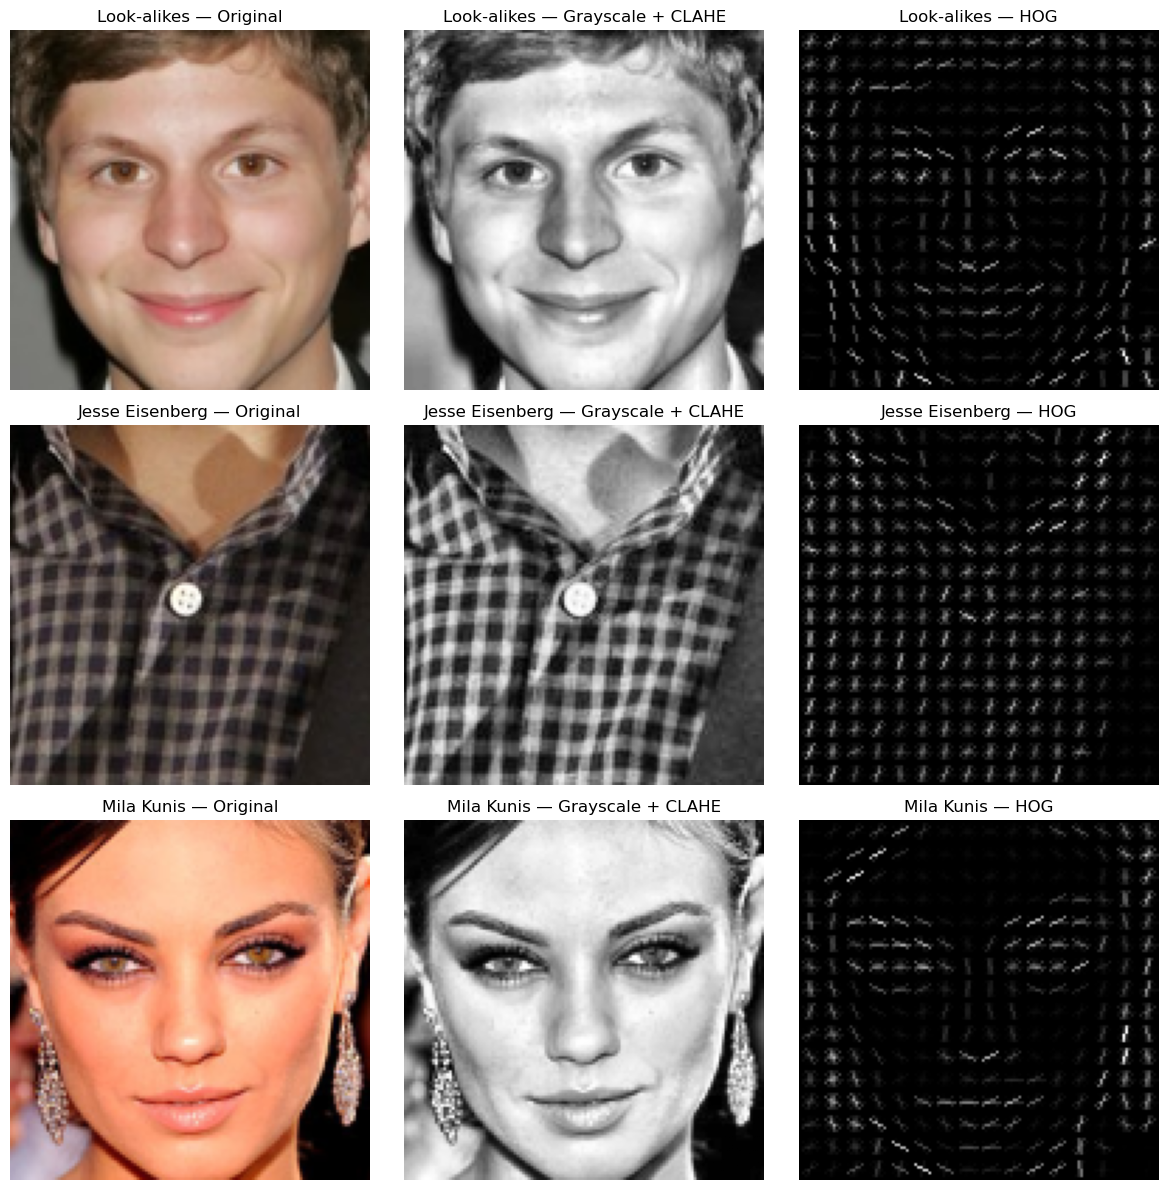
\includegraphics[width=\textwidth]{figures/hog_visualization.png}
    \caption{Four stages of the HOG pipeline for three sample subjects. From left to right: original RGB crop from the HAAR face detector, plain grayscale conversion, grayscale after CLAHE normalization, and the HOG descriptor visualization. CLAHE visibly equalizes lighting. In Jesse Eisenberg's row, the plaid shirt produces strong gradient patterns that dominate the HOG image, illustrating clothing contamination from loose face crops.}
    \label{fig:hog_viz}
\end{figure}

\subsubsection{Face Alignment and Crop Quality}

Our faces are detected and cropped by a HAAR cascade classifier, which finds face-like rectangular regions in images.
This detector does not perform geometric alignment --- it does not rotate tilted faces or ensure that the eyes are always at the same pixel location.
As a result, faces may be slightly shifted, rotated, or scaled differently across images.

HOG is sensitive to these variations because it uses a fixed spatial grid.
If the eyes land in one cell in photo~A but shift two cells to the right in photo~B, the edge patterns will appear in different positions in the HOG vector, and the two photos will look less similar than they actually are.

A second problem is crop tightness.
The HAAR detector sometimes includes substantial neck and shoulder regions.
The HOG visualization (Figure~\ref{fig:hog_viz}) clearly shows this: Jesse Eisenberg's plaid shirt produces strong, regular gradient patterns that dominate his HOG descriptor.
HOG encodes all gradients equally --- it has no way to know that shirt edges are irrelevant and eyebrow edges are important.
This contaminates the feature vector with non-identity information.

\subsubsection{Image Resolution: 128\texttimes128 vs 64\texttimes64}

The face detector crops are resized to a fixed resolution before HOG extraction.
We compare two sizes:

\begin{itemize}
    \item \textbf{Config~A: 128\texttimes128 pixels.} The image is divided into 16$\times$16 = 256 cells, producing an 8\,100-dimensional feature vector. Each cell covers a small patch --- roughly the width of an eyebrow. This fine grid can, in principle, distinguish subtle shape differences like thin versus thick eyebrows or narrow versus wide nose bridges.

    \item \textbf{Config~B: 64\texttimes64 pixels.} The image is divided into 8$\times$8 = 64 cells, producing a 1\,764-dimensional feature vector. Each cell covers a larger area --- roughly an entire eye socket. This coarser grid cannot see fine details, but it is more tolerant of slight face misalignment (because each cell averages over more pixels) and produces far fewer features for the classifier to work with.
\end{itemize}

The trade-off is spatial detail versus robustness.
The finer grid (128\texttimes128) can see more, but what it sees includes noise: skin texture, JPEG compression artifacts, individual clothing fibers.
The coarser grid (64\texttimes64) blurs out these distractions and keeps only the dominant structural edges.
With only 80 training samples, Config~A gives a ratio of 8\,100 features to 80 samples (101:1), while Config~B gives 1\,764 to 80 (22:1).
A classifier working with Config~A has to find meaningful patterns in a space where nearly every direction could be noise.

\subsubsection{HOG Parameter Choices}

Both configurations share the same core HOG settings: 9 orientation bins (spanning 0\textdegree{} to 180\textdegree{} in 20\textdegree{} steps), 8$\times$8 pixels per cell, 2$\times$2 cells per block, and L2-Hys block normalization (the scheme recommended by Dalal and Triggs, which clips extreme gradient values to prevent any single edge from dominating).
These are standard, well-tested defaults.
The only variable we manipulate is the input resolution, which controls how fine the spatial grid is and, consequently, how many features the descriptor produces.

% ---------------------------------------------------------------------------
\subsection{Visualization with t-SNE}

\subsubsection{What t-SNE Does}

Each image in our dataset is now represented as a list of 8\,100 numbers (Config~A) or 1\,764 numbers (Config~B).
We cannot plot a point in 8\,100-dimensional space, so we need a way to compress these numbers down to just two values --- an $x$ and a $y$ coordinate --- that we can plot on a flat page.

t-SNE (t-distributed Stochastic Neighbor Embedding) is a technique designed exactly for this purpose.
Its core idea is: if two images have similar HOG feature vectors, place their dots close together on the 2D plot; if their features are very different, place them far apart.
t-SNE is not a classifier --- it does not try to separate classes.
It simply shows us how the feature vectors are arranged in high-dimensional space, projected down to a flat picture.

t-SNE has one main setting called \textit{perplexity}, which controls how many neighbors each point considers when deciding where to place itself.
Low perplexity (e.g., 5) makes each point care only about its 5 nearest neighbors, revealing tight local clusters.
High perplexity (e.g., 30) makes each point consider 30 neighbors, showing broader global structure but losing fine detail.
We run t-SNE at three perplexity values (5, 15, 30) to see both local and global patterns.

If HOG features were good at distinguishing the three classes, we would see three well-separated clusters of dots, each colored by class.
If HOG features are poor, the dots of different classes will be mixed together with no clear boundaries.

\subsubsection{t-SNE Results}

\paragraph{Separation by class label.}
Figure~\ref{fig:tsne_class} shows 80 dots --- one per training image --- colored by class label (red for Class~0, blue for Class~1, green for Class~2).
At all three perplexity values, the colors are intermixed.
There is no perplexity at which a clear class boundary emerges.
At perplexity~30, the dots compress into a tight blob with all classes on top of each other.
This tells us that HOG feature vectors from different classes are not systematically different --- a classifier would have very little to work with.

\begin{figure}[ht]
    \centering
    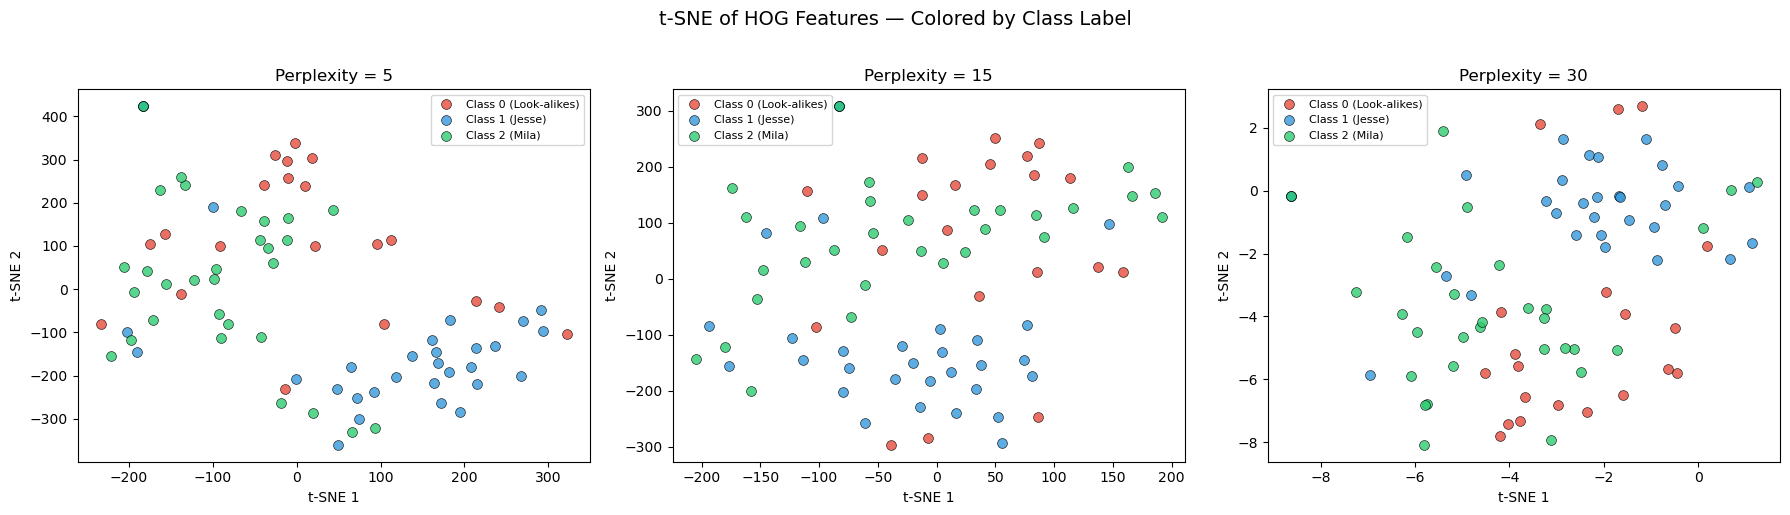
\includegraphics[width=\textwidth]{figures/tsne_by_class.png}
    \caption{t-SNE of HOG features (Config~A, 8\,100 dims) colored by class label at perplexity 5, 15, and 30. All three classes remain intermixed at every scale. No clean separation is visible.}
    \label{fig:tsne_class}
\end{figure}

\paragraph{Separation by identity.}
Figure~\ref{fig:tsne_identity} re-colors the same embeddings by the four actual identities: Jesse Eisenberg, Michael Cera, Mila Kunis, and Sarah Hyland.
The male look-alike pair (Jesse and Michael) overlaps almost completely at all perplexity values.
The female pair (Mila and Sarah) shows a similar pattern.
A faint gender-related trend is visible at perplexity~15 --- male subjects drift slightly toward one side, female subjects toward the other --- but this separation is far too weak and inconsistent to be useful for classification.

\begin{figure}[ht]
    \centering
    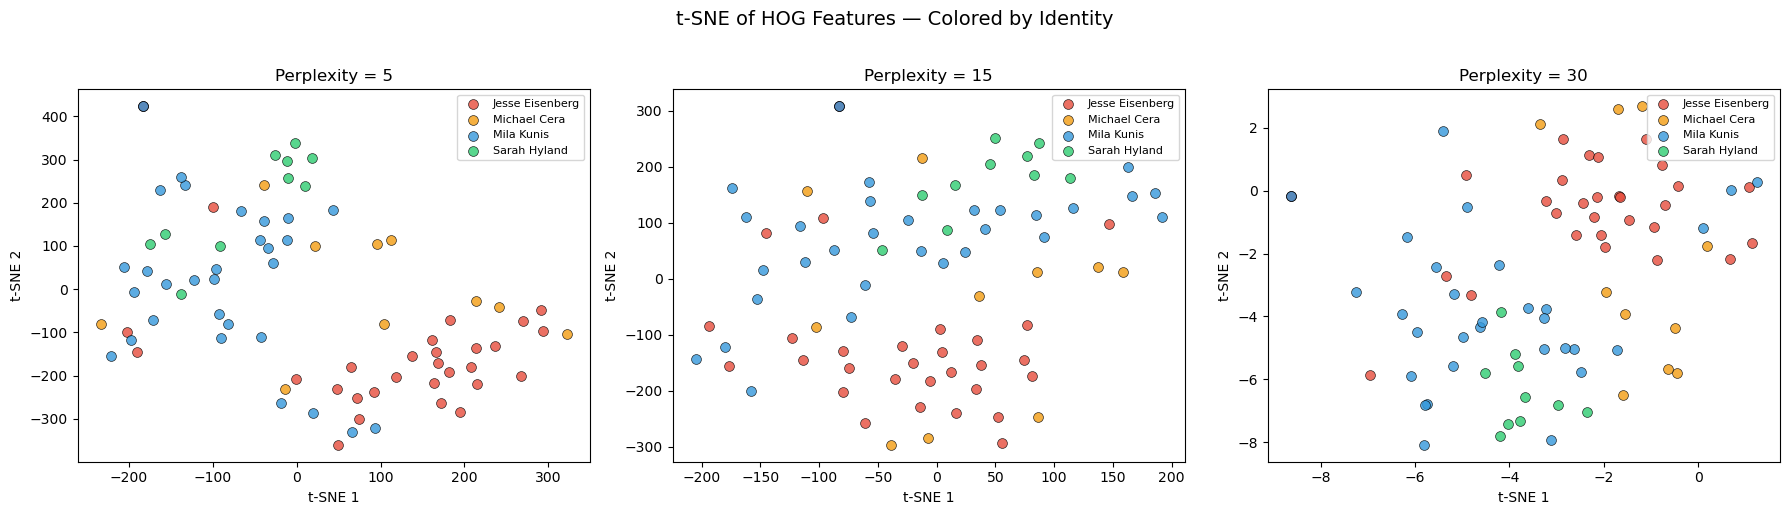
\includegraphics[width=\textwidth]{figures/tsne_by_identity.png}
    \caption{t-SNE of HOG features colored by identity. Look-alike pairs (Jesse/Michael, Mila/Sarah) overlap heavily, confirming that HOG captures the shared facial geometry that makes them look alike.}
    \label{fig:tsne_identity}
\end{figure}

\paragraph{Config~A versus Config~B.}
Figure~\ref{fig:config_ab} compares the two resolution configurations side by side at perplexity~15.
Config~A (128\texttimes128, 8\,100 dimensions) and Config~B (64\texttimes64, 1\,764 dimensions) produce nearly identical t-SNE structure: the same loose, overlapping clusters with no clean class boundaries.
This is the key result of the resolution comparison.
If the extra spatial detail in Config~A carried useful identity information, we would see tighter same-class clusters and wider gaps between classes on the left plot compared to the right.
Instead, both look equally disorganized, confirming that the extra 6\,336 dimensions in Config~A mostly encode noise --- skin texture, compression artifacts, clothing threads --- rather than discriminative facial structure.
Given the small dataset (80 samples), Config~B's 22:1 feature-to-sample ratio is strongly preferable to Config~A's 101:1.

\begin{figure}[ht]
    \centering
    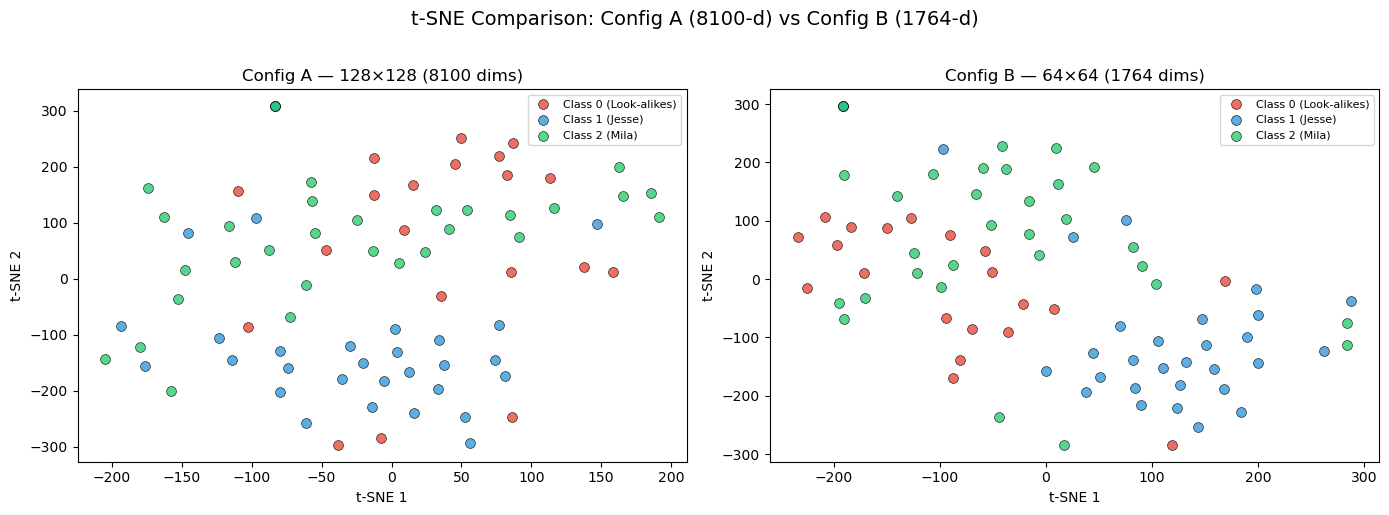
\includegraphics[width=\textwidth]{figures/config_a_vs_b.png}
    \caption{Side-by-side t-SNE comparison at perplexity~15. Left: Config~A (128\texttimes128, 8\,100 dims). Right: Config~B (64\texttimes64, 1\,764 dims). The cluster structure is virtually identical, showing that the extra resolution does not improve class separation.}
    \label{fig:config_ab}
\end{figure}

% ---------------------------------------------------------------------------
\subsection{Main HOG Findings}

The HOG experiments lead to three conclusions:

\begin{enumerate}
    \item \textbf{HOG features have weak discriminative power for look-alike faces.} The t-SNE visualizations show no clean class separation at any perplexity. HOG encodes coarse facial shape, which is exactly the property that look-alike pairs share. This makes HOG fundamentally limited for this specific task.

    \item \textbf{Higher image resolution does not help.} Config~A (128\texttimes128) and Config~B (64\texttimes64) produce equivalent t-SNE structure. The finer spatial grid does not capture additional identity-discriminative information; it mostly amplifies noise. With only 80 training samples, the more compact Config~B is the better choice.

    \item \textbf{Crop quality matters as much as the descriptor.} The HAAR face detector includes non-face regions (neck, clothing) in many crops. Since HOG treats all gradients equally, clothing patterns contaminate the feature vector. A tighter, more precise face detector or a face-alignment step would likely improve results even without changing the descriptor.
\end{enumerate}

% ---------------------------------------------------------------------------
\subsection{Limitations}

Several limitations prevent HOG from performing well on this task:

\begin{itemize}
    \item \textbf{Fixed spatial grid.} HOG divides the image into a rigid, uniform grid. It cannot focus attention on informative regions (eyes, mouth) or ignore uninformative ones (forehead, background). Every patch gets equal weight.

    \item \textbf{No geometric invariance.} HOG assumes the face is upright and centered. It has no built-in mechanism to handle rotation, scale changes, or shifts in face position. Unlike keypoint-based descriptors (such as SIFT), HOG cannot adapt to local geometric deformations.

    \item \textbf{Curse of dimensionality.} Even with Config~B, the 1\,764-dimensional feature vector is large relative to 80 training samples. A classifier must work in a space where most directions are noise, making it difficult to learn robust decision boundaries.

    \item \textbf{Clothing and background contamination.} The HAAR detector's loose crops include non-face content. HOG indiscriminately encodes gradients from clothing, hair, and background alongside actual facial structure.
\end{itemize}

% ---------------------------------------------------------------------------
\subsection{Possible Future Improvements for HOG}

Several directions could address the HOG-specific limitations identified above:

\begin{itemize}
    \item \textbf{Face alignment.} Using a landmark detector (e.g., dlib's 68-point model) to align faces before cropping would ensure that eyes, nose, and mouth are always at the same pixel coordinates. This would make HOG features more consistent across different photos of the same person.

    \item \textbf{Tighter crops.} Masking or cropping out non-face regions (below the chin, above the hairline) would eliminate clothing and background contamination.

    \item \textbf{Dimensionality reduction.} Applying PCA to the HOG features before classification could remove noisy dimensions and improve the feature-to-sample ratio, potentially rescuing some discriminative signal.
\end{itemize}

% ===========================================================================
\section{SIFT: Scale-Invariant Feature Transform}
% ===========================================================================

Having established that HOG features lack discriminative power for look-alike faces, we now evaluate a second handcrafted descriptor: the Scale-Invariant Feature Transform (SIFT), introduced by Lowe (2004).

% ---------------------------------------------------------------------------
\subsection{How SIFT Works}

SIFT detects and describes local image regions called \textit{keypoints}.
Each keypoint is identified in a Difference-of-Gaussian (DoG) scale-space pyramid, which makes its detection inherently invariant to the scale (size) of the object in the image.
For each keypoint, a dominant gradient orientation is assigned, providing rotation invariance.
The descriptor itself encodes the gradient structure in a 16$\times$16 pixel neighborhood around the keypoint, subdivided into a 4$\times$4 grid of sub-regions with 8 orientation bins each, yielding a 128-dimensional vector per keypoint.

The key difference from HOG is locality: SIFT describes \textit{individual image patches} rather than the entire image, and its descriptors are invariant to scale and rotation by construction.

% ---------------------------------------------------------------------------
\subsection{Dense SIFT for Face Images}

Standard SIFT relies on automatic keypoint detection, which identifies corners, blobs, and other high-contrast regions.
On face images, this is problematic: faces are relatively smooth surfaces with few strong corners, and automatically detected keypoints tend to cluster on eyebrows and nostrils while ignoring equally informative regions such as the cheek contour or chin.
The number of detected keypoints also varies across images, producing variable-length descriptors.

We therefore use a \textbf{dense SIFT} strategy: a regular grid of keypoints is placed across the entire image at fixed 4-pixel intervals.
This ensures that descriptors are extracted from consistent facial regions across all samples and that every image produces the same number of descriptors.

\subsubsection{Preprocessing}

The preprocessing pipeline mirrors the HOG approach: images are converted to grayscale, resized to 64$\times$64 pixels, and processed with CLAHE to normalize illumination.
Any failed face detections (NaN pixels) are replaced with zeros.

\subsubsection{Feature Aggregation}

Since each image produces many local 128-dimensional descriptors (one per grid point), we aggregate them into a fixed-length representation by computing the \textbf{mean} and \textbf{standard deviation} across all descriptors and concatenating them.
This yields a compact \textbf{256-dimensional} feature vector per image (128 mean + 128 std).
The mean captures the dominant gradient structure of the face; the standard deviation captures how much that structure varies spatially --- a proxy for texture complexity.

This representation has a feature-to-sample ratio of only 3.2:1 on our 80 training samples, compared to HOG's 101:1 (Config~A) or 22:1 (Config~B).

\subsubsection{Parameter Choices}

The dense grid uses a step size of 4~pixels and a keypoint neighborhood size of 6~pixels, balancing spatial coverage against robustness to small appearance variations.
CLAHE is enabled with the same settings used for HOG (clip limit 2.0, tile grid 8$\times$8).

% ---------------------------------------------------------------------------
\subsection{SIFT t-SNE Results}

Before running t-SNE, the 256-dimensional SIFT features are standardized (zero mean, unit variance) and reduced to 20 principal components with PCA.
Standardization prevents dimensions with larger magnitudes from dominating the distance metric, and PCA removes linear redundancies.

The t-SNE projection shows only a \textbf{marginal improvement} over the HOG results.
Class~2 (Mila Kunis) has a slight tendency to appear in the upper portion of the embedding, and Class~1 (Jesse Eisenberg) drifts toward the lower-right, but all three classes overlap heavily across the entire plot.
No region is clearly dominated by a single class.
Compared to HOG's complete intermixing, the SIFT embedding exhibits a faint vertical stratification, suggesting that the SIFT representation captures a weak but nonzero class-related signal.
However, the separation is far too noisy to call meaningful on its own.

% ===========================================================================
\section{SIFT vs HOG: Comparison and Recommendation}
% ===========================================================================

% ---------------------------------------------------------------------------
\subsection{Side-by-Side Comparison}

\begin{table}[ht]
\centering
\begin{tabular}{l l l}
\hline
\textbf{Criterion} & \textbf{HOG} & \textbf{Dense SIFT} \\
\hline
Feature type & Fixed-grid edge histograms & Local keypoint descriptors \\
Dimensionality & 8{,}100 / 1{,}764 & 256 \\
Dims:samples ratio & 101:1 / 22:1 & 3.2:1 \\
Scale invariance & None & Inherent (DoG pyramid) \\
Rotation invariance & None & Partial (orientation assignment) \\
Illumination robustness & CLAHE + L2-Hys & CLAHE + per-descriptor norm \\
Misalignment sensitivity & High (fixed grid) & Low (aggregate statistics) \\
t-SNE class separation & None & Marginal \\
Clothing contamination & Severe & Mild (diluted by averaging) \\
\hline
\end{tabular}
\caption{Comparison of HOG and dense SIFT descriptors on the look-alike face recognition task.}
\label{tab:sift_vs_hog}
\end{table}

% ---------------------------------------------------------------------------
\subsection{Theoretical Advantages of SIFT}

Although the t-SNE evidence is inconclusive, three theoretical properties suggest that SIFT should be better suited to fine-grained face discrimination:

\begin{enumerate}
    \item \textbf{Local, multi-scale descriptors.} Each SIFT descriptor encodes gradients in a 16$\times$16 neighborhood with 4$\times$4 spatial binning.
    This multi-resolution structure captures fine texture and micro-geometry (e.g., the curvature around the eye socket, the gradient pattern at the hairline) that HOG's coarser 8$\times$8 cell grid averages away.

    \item \textbf{Compact representation.} The 256-dimensional feature vector gives a 3.2:1 feature-to-sample ratio, dramatically reducing overfitting risk compared to HOG.
    The signal-to-noise ratio in the feature space remains high.

    \item \textbf{Robustness to misalignment and contamination.} By aggregating descriptors with mean and standard deviation, the representation becomes insensitive to the exact spatial position of features.
    A slight shift in face alignment or a few keypoints falling on clothing contribute minimally to the aggregate.
    HOG, by contrast, encodes each cell at a fixed location, so any spatial shift corrupts the entire vector.
\end{enumerate}

% ---------------------------------------------------------------------------
\subsection{Recommendation}

\textbf{Neither descriptor achieves reliable class separation on this look-alike dataset, but dense SIFT is the more promising starting point for downstream classification.}

The t-SNE visualizations reveal the difficulty of this task for handcrafted features: HOG embeddings show complete class intermixing at all perplexities, while SIFT embeddings show only a marginal improvement --- a faint tendency for classes to occupy different vertical bands, but with heavy overlap throughout.
On visual evidence alone, neither descriptor is convincing.

The recommendation for SIFT therefore rests primarily on theoretical grounds.
Its 256-dimensional representation yields a 3.2:1 feature-to-sample ratio, compared to HOG's 22:1 (Config~B) or 101:1 (Config~A), substantially reducing the risk of overfitting with only 80 training samples.
SIFT's built-in scale and partial rotation invariance make it more tolerant of the inconsistent crops produced by the HAAR face detector, and its mean/standard-deviation aggregation dilutes contamination from clothing or background regions that severely affects HOG's fixed grid.
These properties make SIFT more likely to generalize to unseen data, even when t-SNE does not show dramatic cluster separation.

HOG retains value for coarse shape discrimination tasks (face detection, gender classification) and could serve as a complementary feature in an ensemble.
However, for fine-grained look-alike discrimination with limited training data, SIFT offers a better trade-off between descriptive power and statistical robustness.

Reliable look-alike recognition with handcrafted features would likely require richer aggregation schemes (Fisher vectors, VLAD), explicit face alignment with landmark detectors, or a combination of both descriptors.
Learned representations from pre-trained deep networks (FaceNet, ArcFace) offer a fundamentally different approach, though they fall outside the scope of handcrafted features.

\end{document}
